\chapter{修士作品 《Grasp(er)》}
\label{about_grasper}
本章では、修士作品《Grasp(er)》の作品概要と、作品におけるねらいをSidney Felsが定義したembodimentの分類に基づいて示す。

\section{作品概要}
\begin{figure}[H]
  \centering
  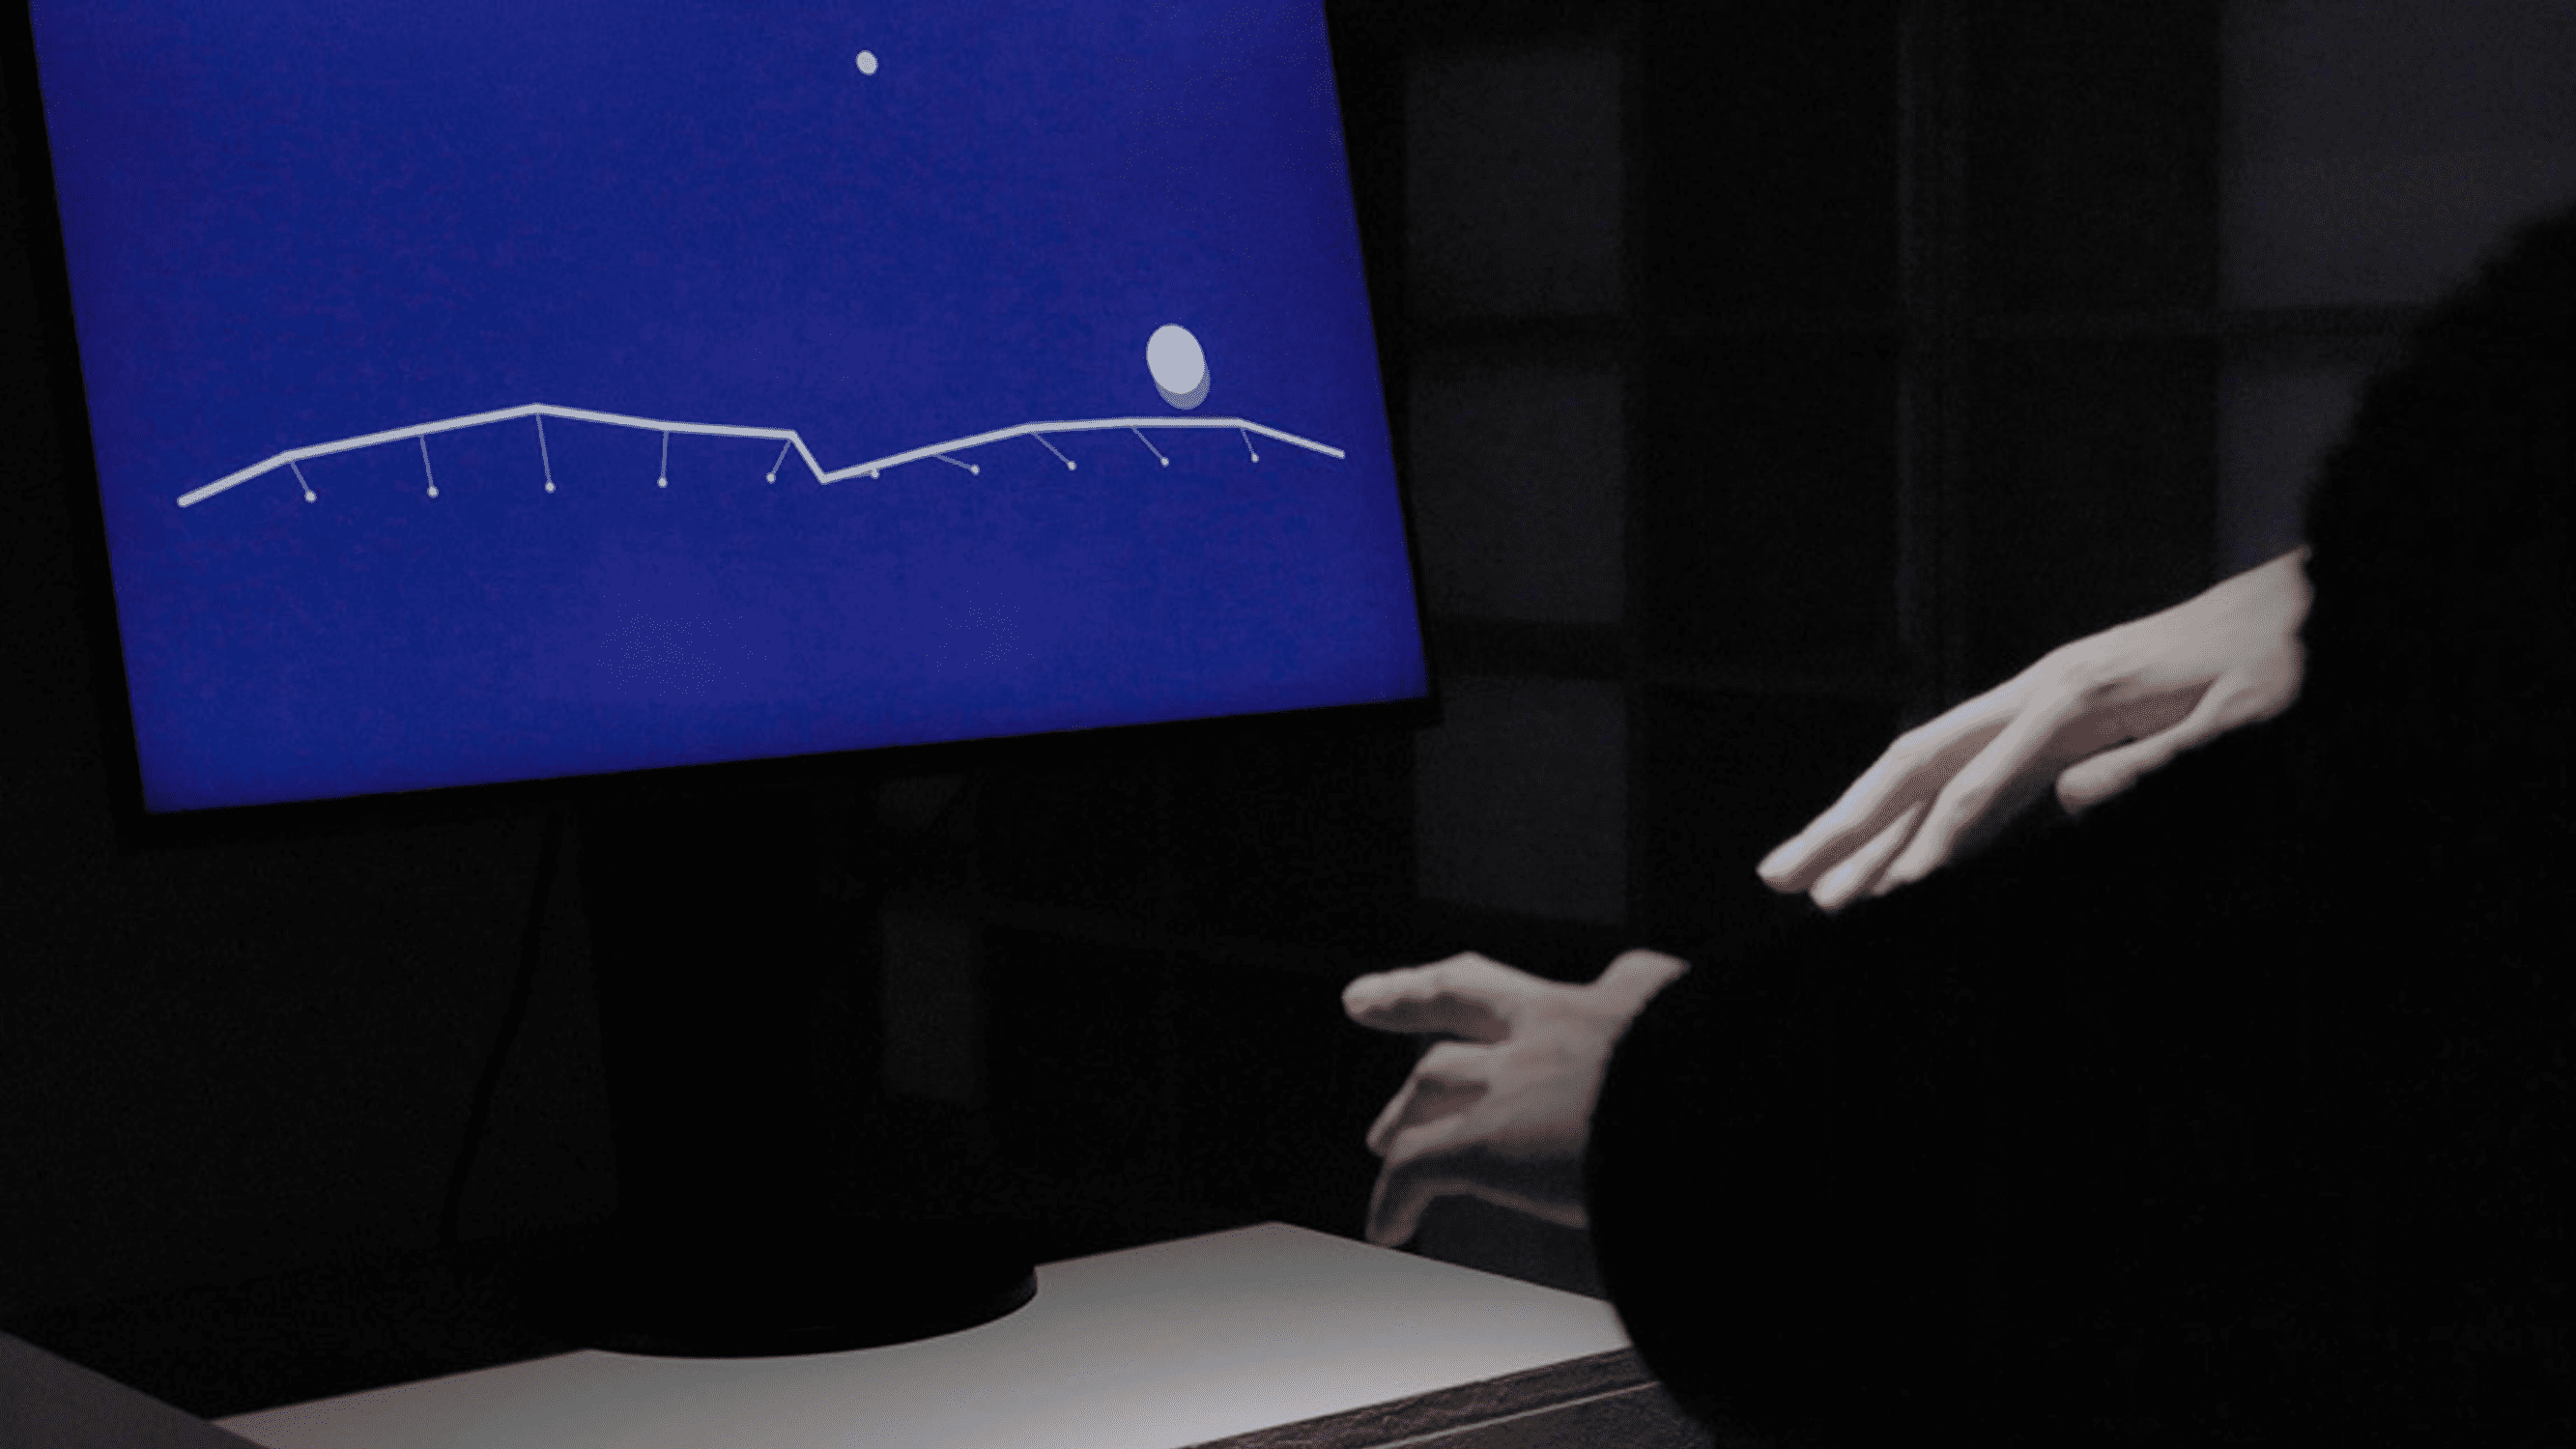
\includegraphics[width=15cm]{img/thumbnail.png}
  \caption{修士作品《Grasp(er)》}
  \label{grasper}
\end{figure}

《Grasp(er)》は、「Familiar / Strange」と「Relation」という二つから構成された作品群である。最初は鏡合わせのように映った手の形が大きく変化する中で、自身の身体と手指の関係がわからなくなりながらも、注意を向けて探索的に手指を動かしていると、体の動きと画面の中の動きが一致するような感覚が芽生える。また、形の変わった手指を使って緻密な動きをする中、最初はうまくいかずもどかしさを感じながらも、試行錯誤を経て一体感が芽生えるようになる。このように《Grasp(er)》では、体験の中で意識的に調和する感覚を掴み取り、一体となる感覚を目指した。

以下では、本作を構成する2つの作品について説明する。

% これらに共通するのは、\textit{grasp}の中で個人が目的意識や興味を抱くことで、\textit{grasp}が連鎖的に生じることである。

% 制作者は「このようなことをしてほしい」という行為の中身を設計せず、体験する個人がその中で次々と注目する対象を見出すことによって、個人が行為を創造していくことを目指している。このため、「手指の構造や、手指を取り巻く環境を変化させることで、手指の運動に注目する構造」を作ることに取り組んだ。このときの「注目」が起点となって\textit{grasp}の期間が生じるが、その先々で起こる体験は個人に委ねられ、明示的な目的は設定されていない。

\subsection*{Familiar / Strange}
\begin{figure}[H]
  \centering
  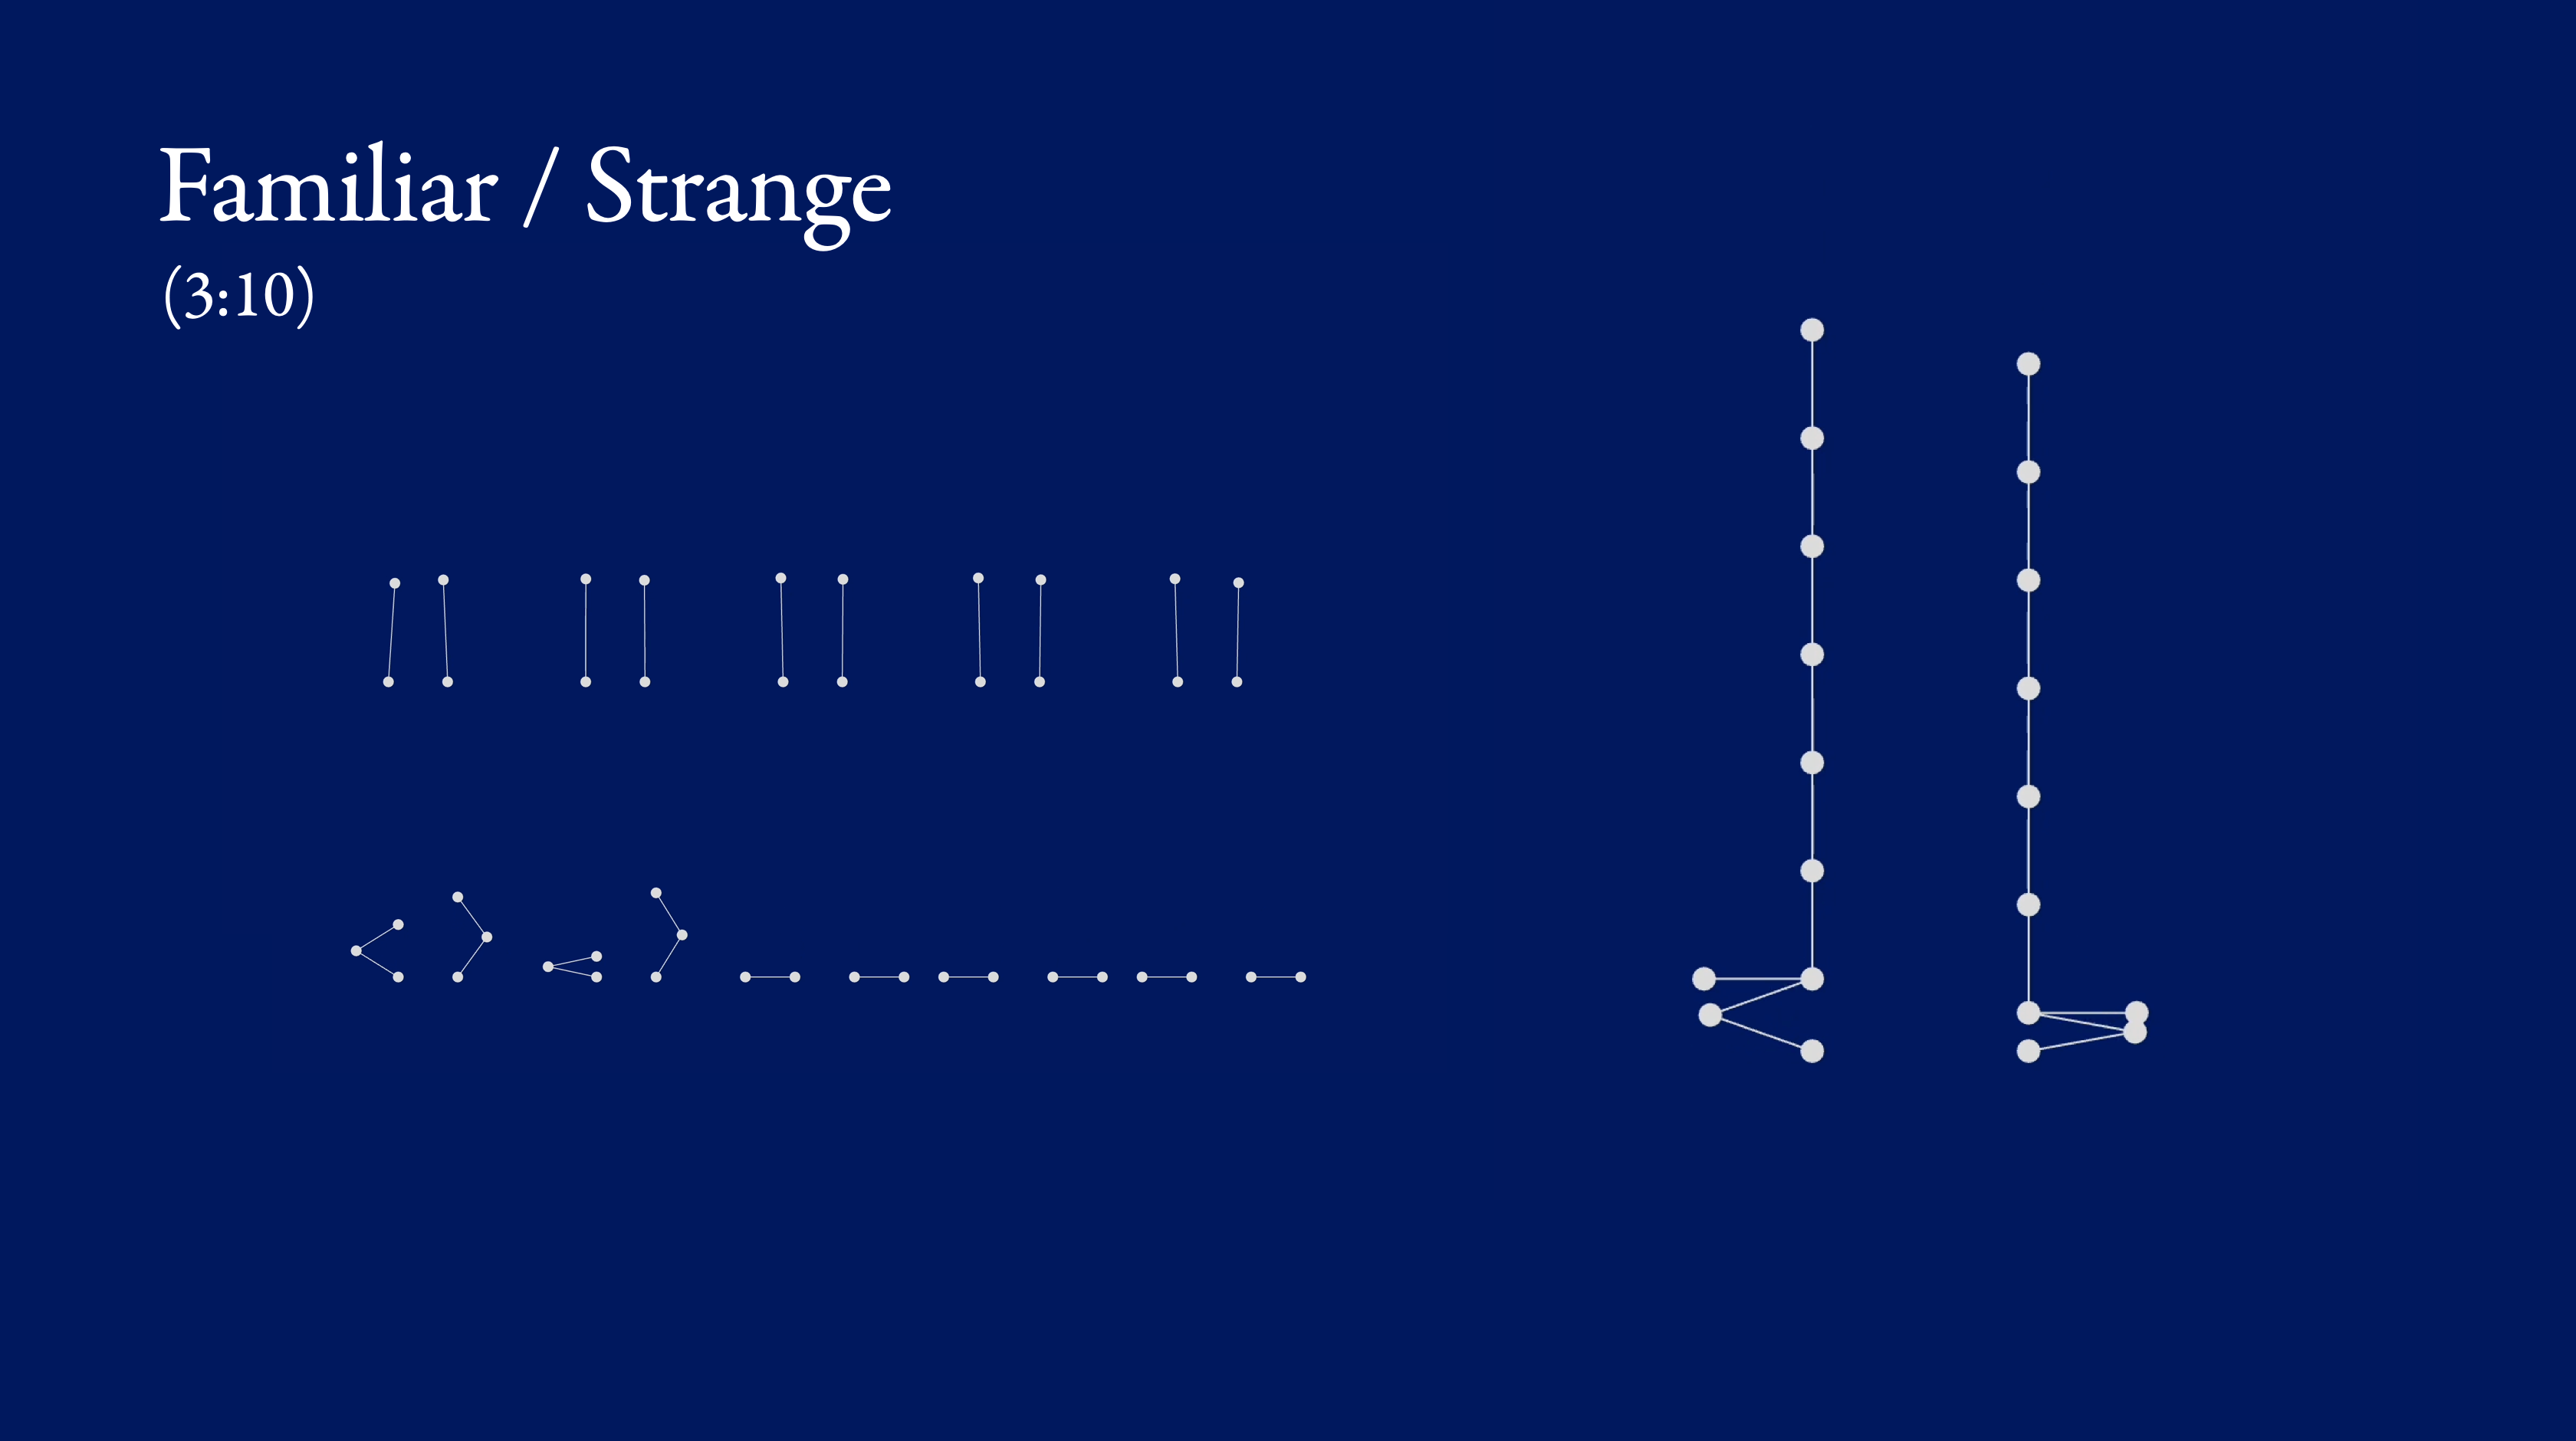
\includegraphics[width=15cm]{img/fs-02.png}
  \caption{Familiar / Strange}
  \label{fig:familiar_strange}
\end{figure}
「Familiar / Strange」は、手指の配置や関節の数・位置が次々と変化していく作品で、手の運動に対する再注目が起きることを目指している。作品は最初、手の形がそのまま現れた状態から開始し、指の並びや関節の配置の変化が起きる。一本一本の指がくの字の形をして積み上げられる様子をピークに、逆順に変化が巻き戻され、再び元の手の形に戻るという、3分10秒で1ループの構造となっている。変換の過程は、イージングやゴム紐が切れた時のような振動を伴う動きによって補完される。

\subsection*{Relation}
\begin{figure}[H]
  \centering
  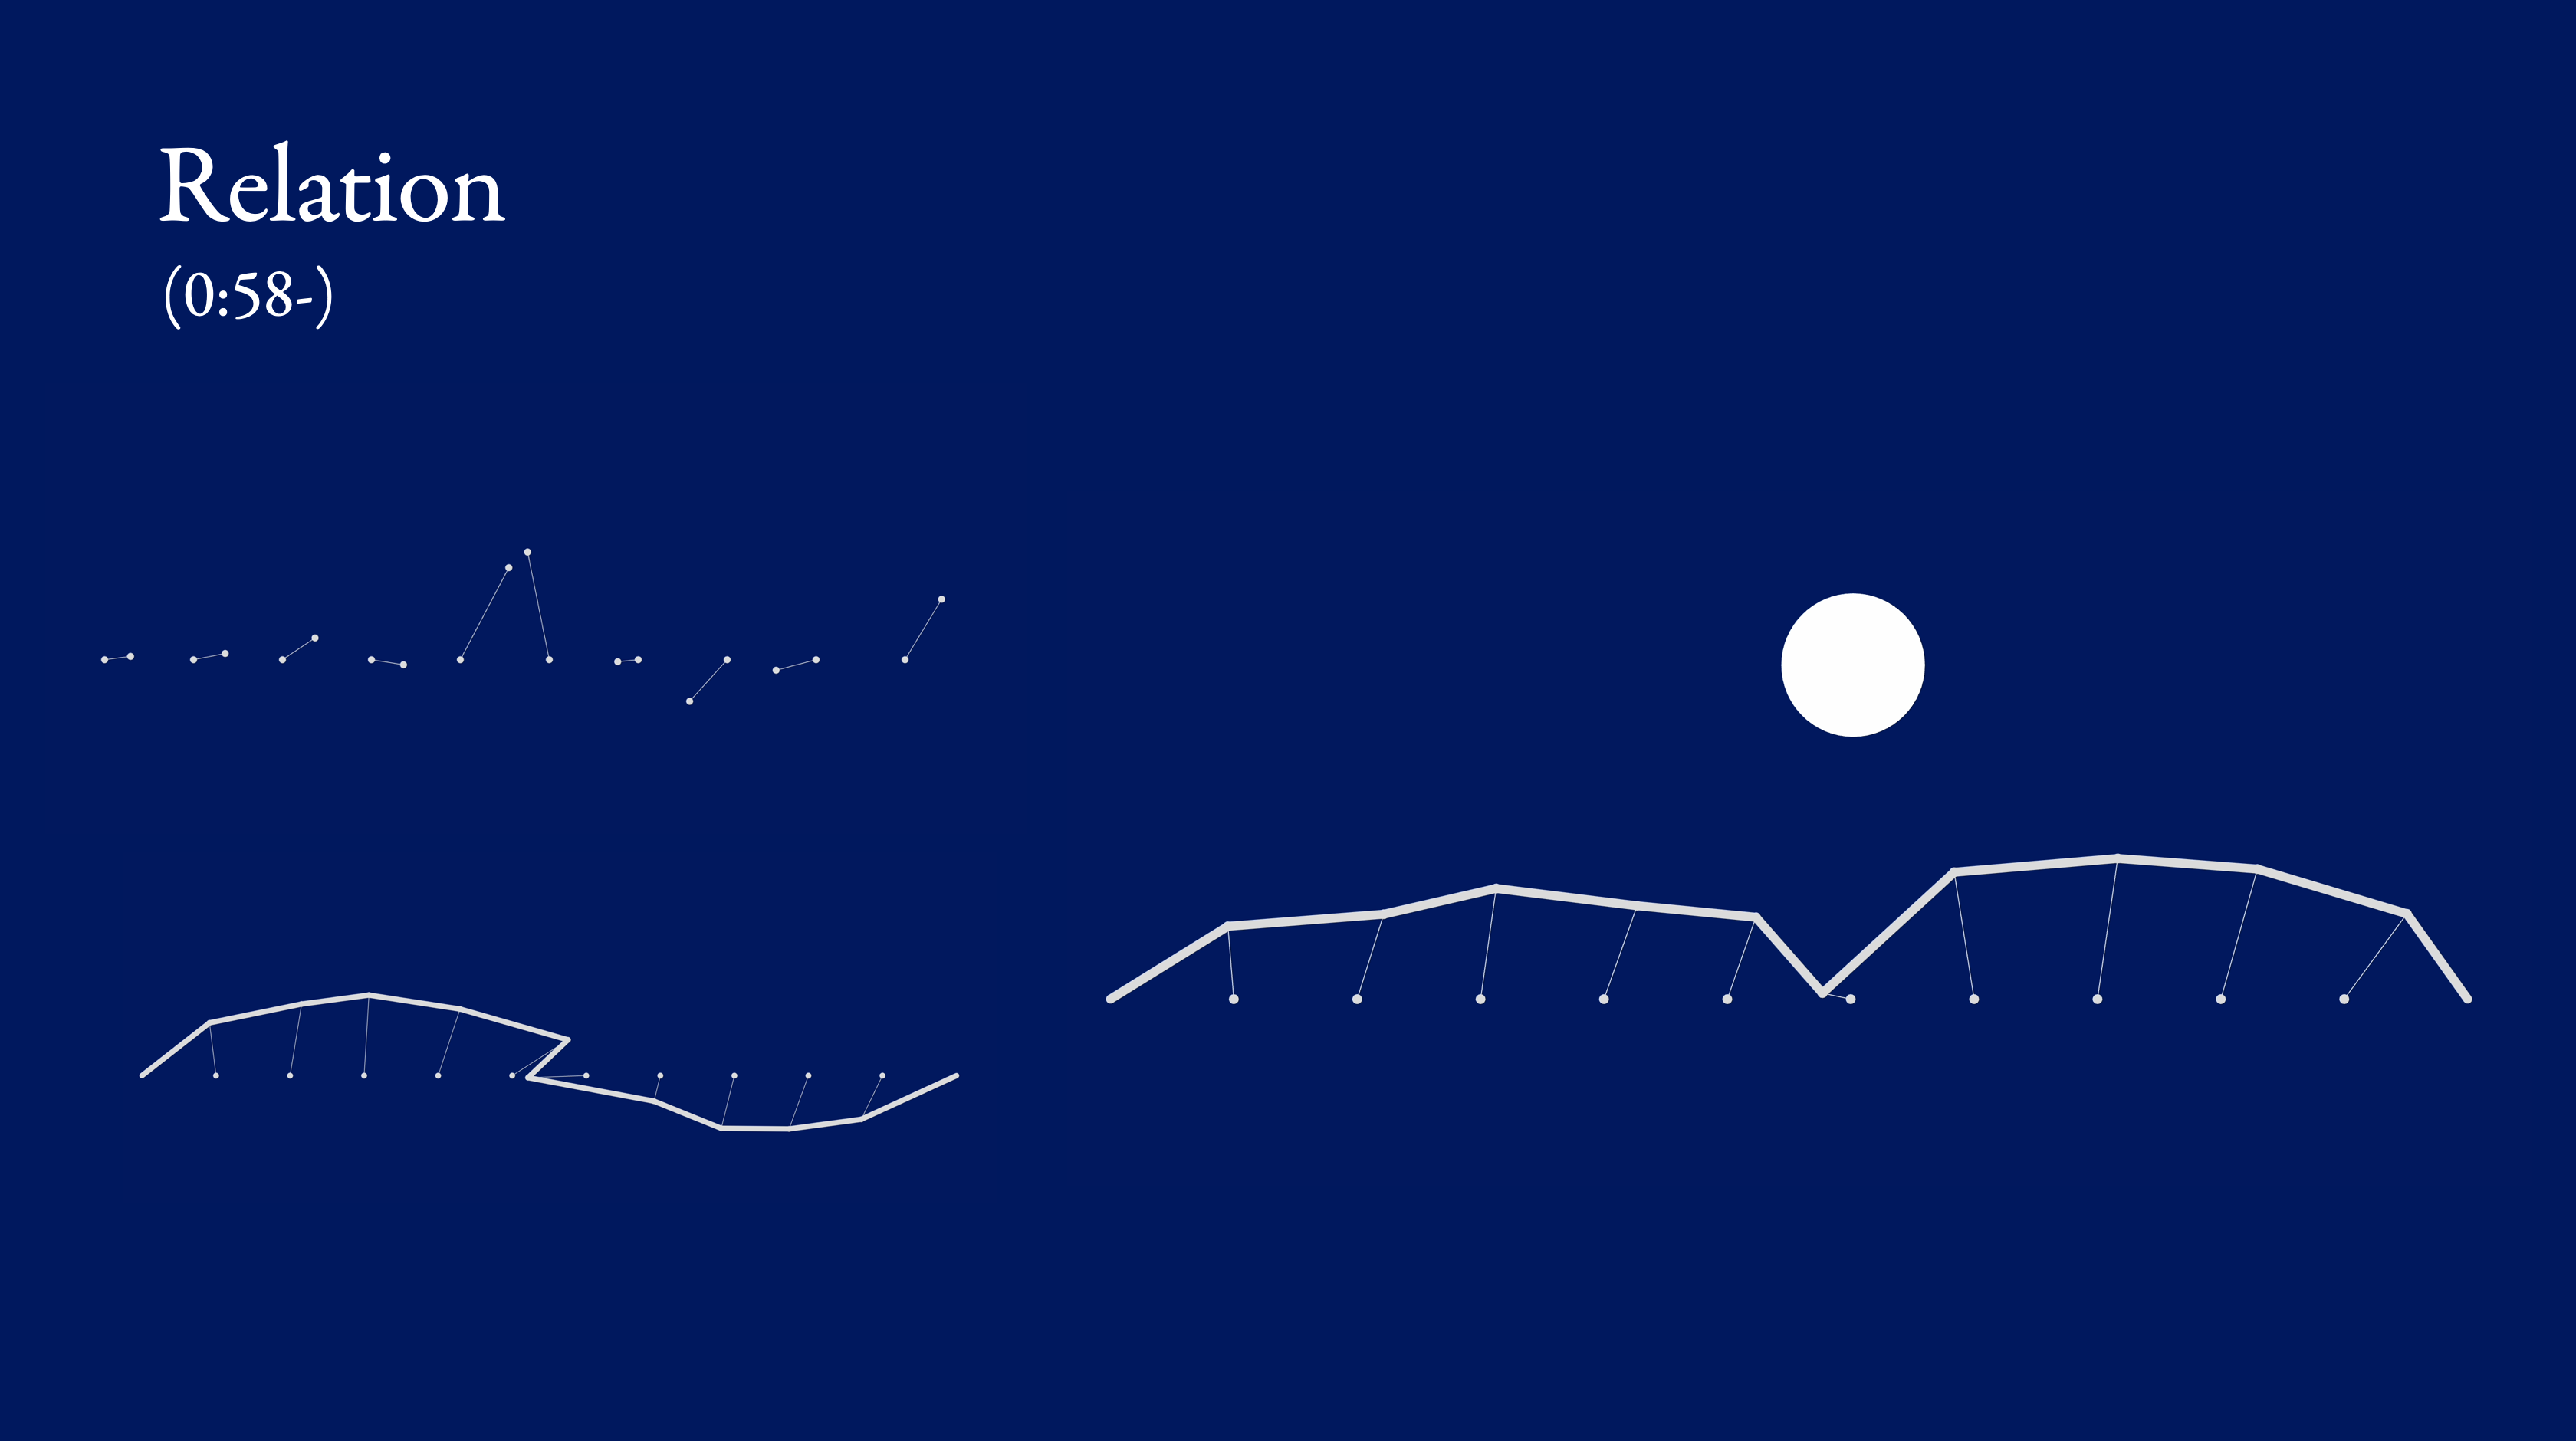
\includegraphics[width=15cm]{img/relation.png}
  \caption{Relation}
  \label{fig:relation}
\end{figure}
「Relation」は、変化した手指を取り巻く関係が次々と変化していく作品で、手と直接的に制御できないボールの関係に焦点を当てている。1つ目の作品と同様、最初は手が表示された状態から始まり、段階的に並び替えられた手指を覆う皮膜が現れ、ボールが現れる。最後はマトが現れ、マトを取るたびにボールの大きさが小さくなり、3つ連続してマトにあたったとき、皮膜は消え、再び元の手の形に戻る。

トラッキングされた手指の位置が、手首から指ごとに分割され、左端から右へ、左手の小指から親指、そして右手の親指から小指の順に整列される。しばらくすると、指先以外の運動が捨象され、残された指先を結ぶ線が現れる。ここで、現れた線によって再び全ての指が1つのまとまりとして統合されることになるが、その線は後に現れるボールに対して衝突判定が適用される、新しい構造の手指を覆う皮膜のような機能を有する。皮膜のある領域を外れるとボールは落下するが、そのあとは再び画面の中央にボールが出現する。

さらに一定時間が経過すると、皮膜の上方に白い点:マトが現れる。マトに対してボールを当てると、ボールは一回り小さくなり、ボールを落とさずに合計3回マトに当てることでボールは消失し、皮膜が現れるときと逆の順序を辿って画面の中の手は再びもとの形状に戻る。

\section{作品体験のねらい}
\label{nerai}
本作について、Felsのカテゴリをもとに作品体験のねらいを説明する。

\subsection*{Familiar / Strange}
この作品におけるねらいは、トランジションの際の違和感が起点となって意識的な試行が引き出され、身体動作が変化することで一体感が生起することである。以下の説明では、便宜上図\ref{fig:diagram_familiar_strange}のように、それぞれのシーンに対して番号を割り当てる。その上で、図\ref{fig:nerai_fs}に、本作品におけるねらいを図示した(数字はシーン番号)。

\begin{figure}[H]
  \centering
  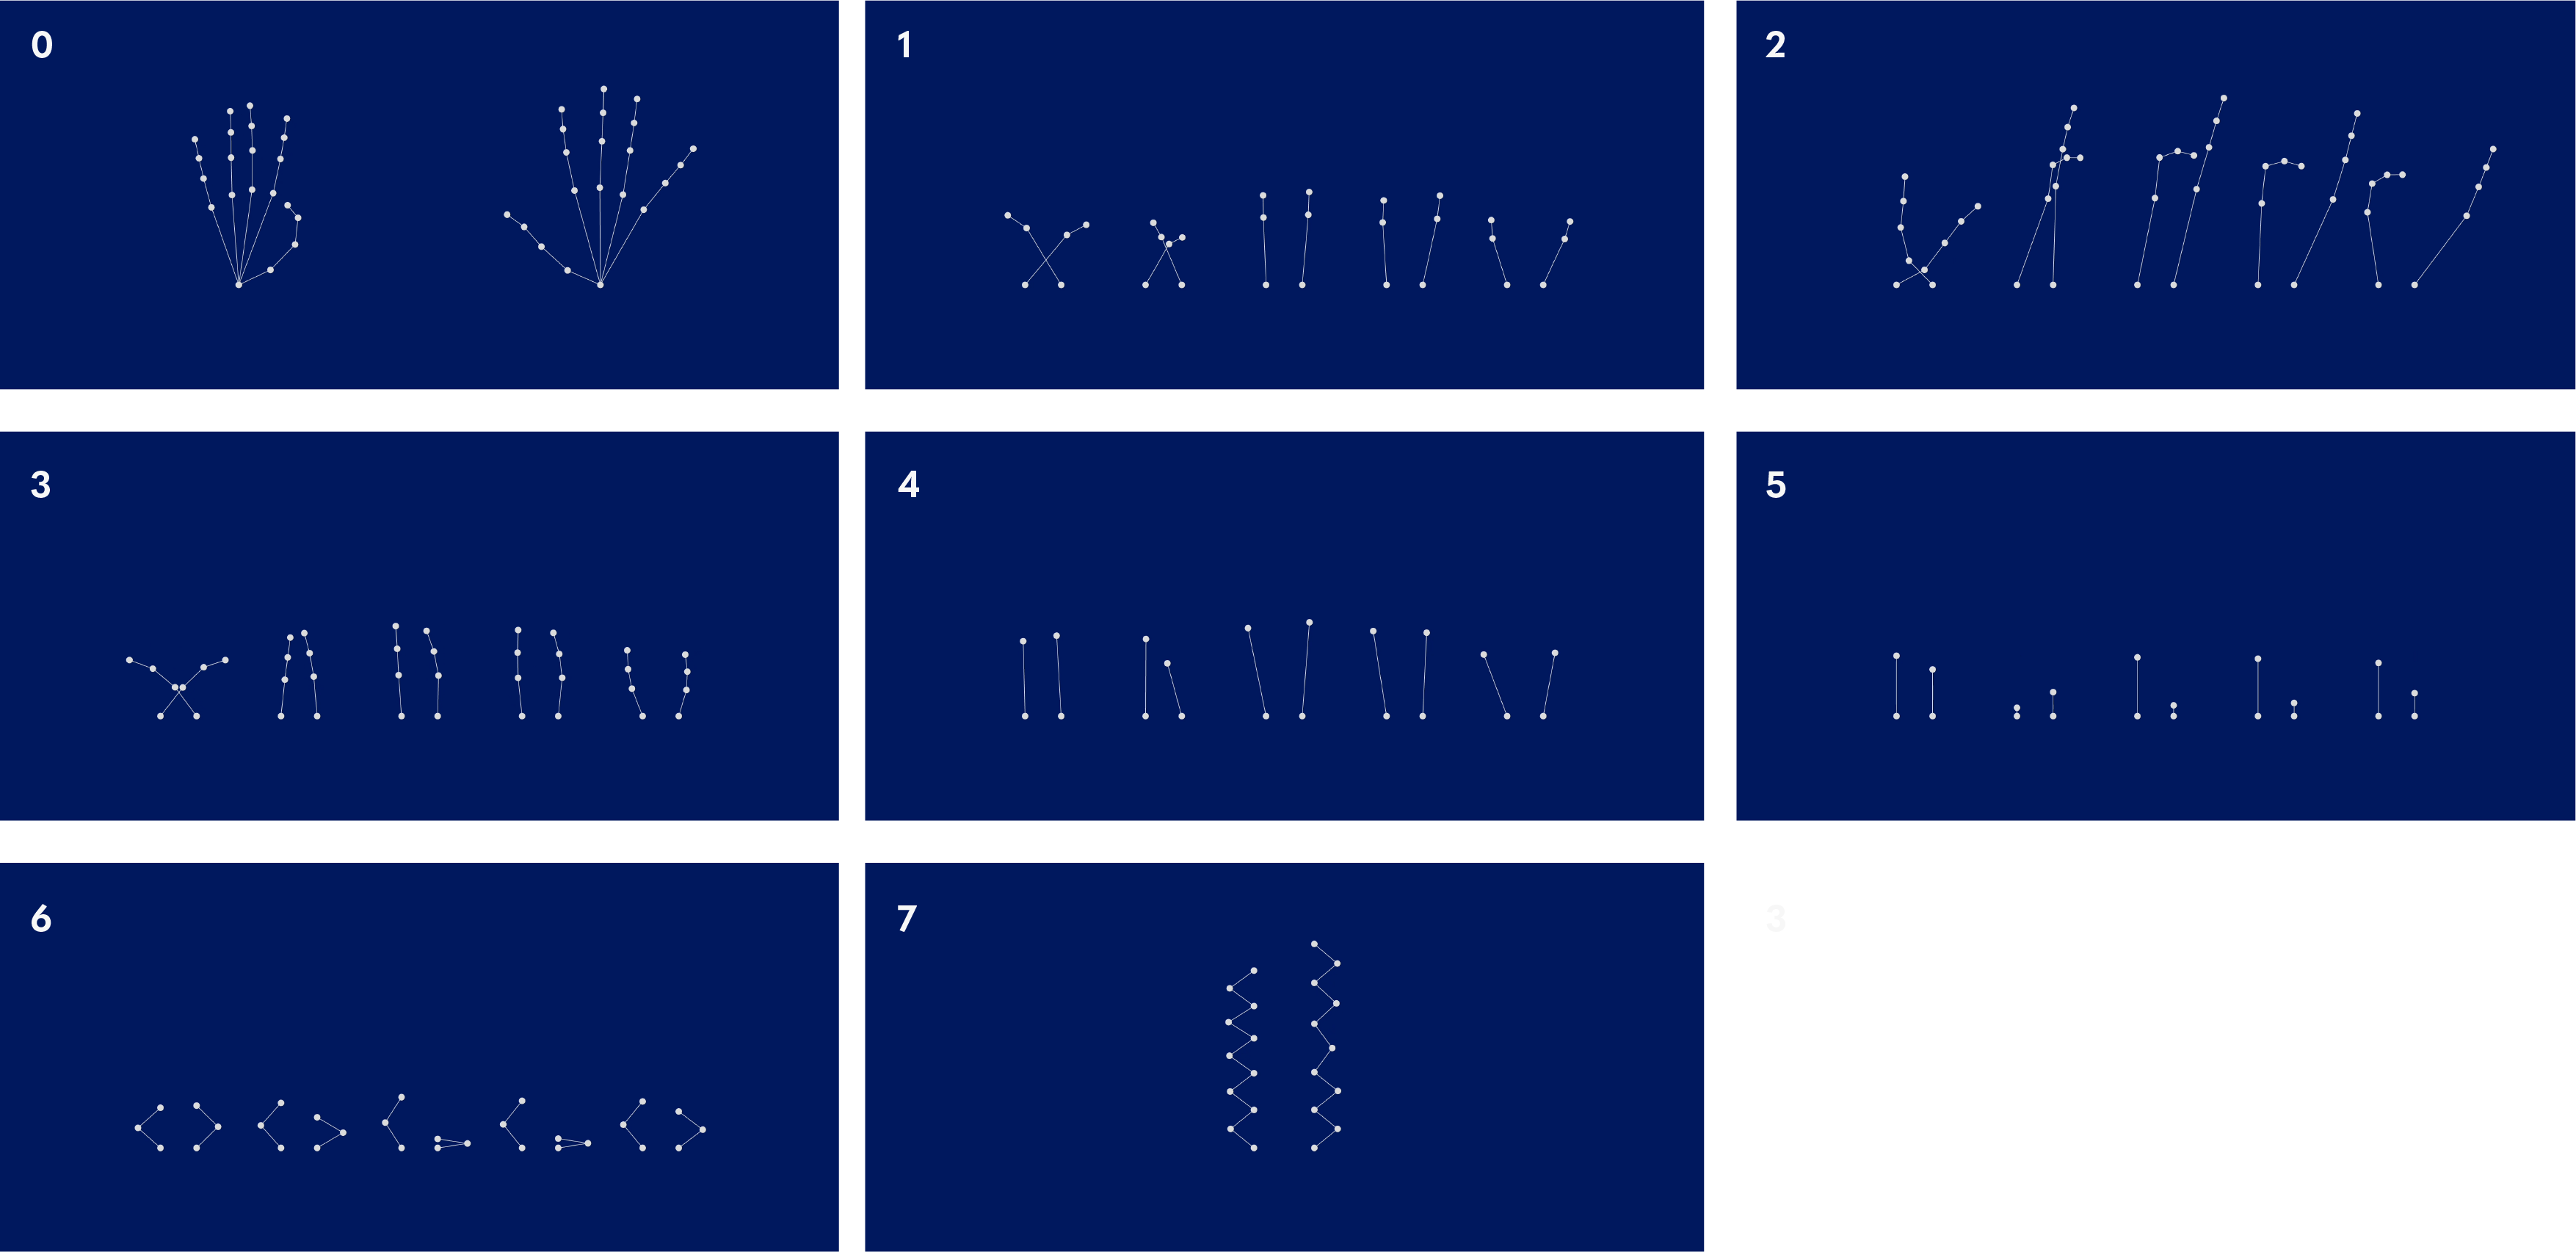
\includegraphics[width=15cm]{img/handpose-sequence.png}
  \caption{Familiar / Strangeにおけるシーン遷移}
  \label{fig:diagram_familiar_strange}
\end{figure}

\begin{figure}[H]
  \centering
  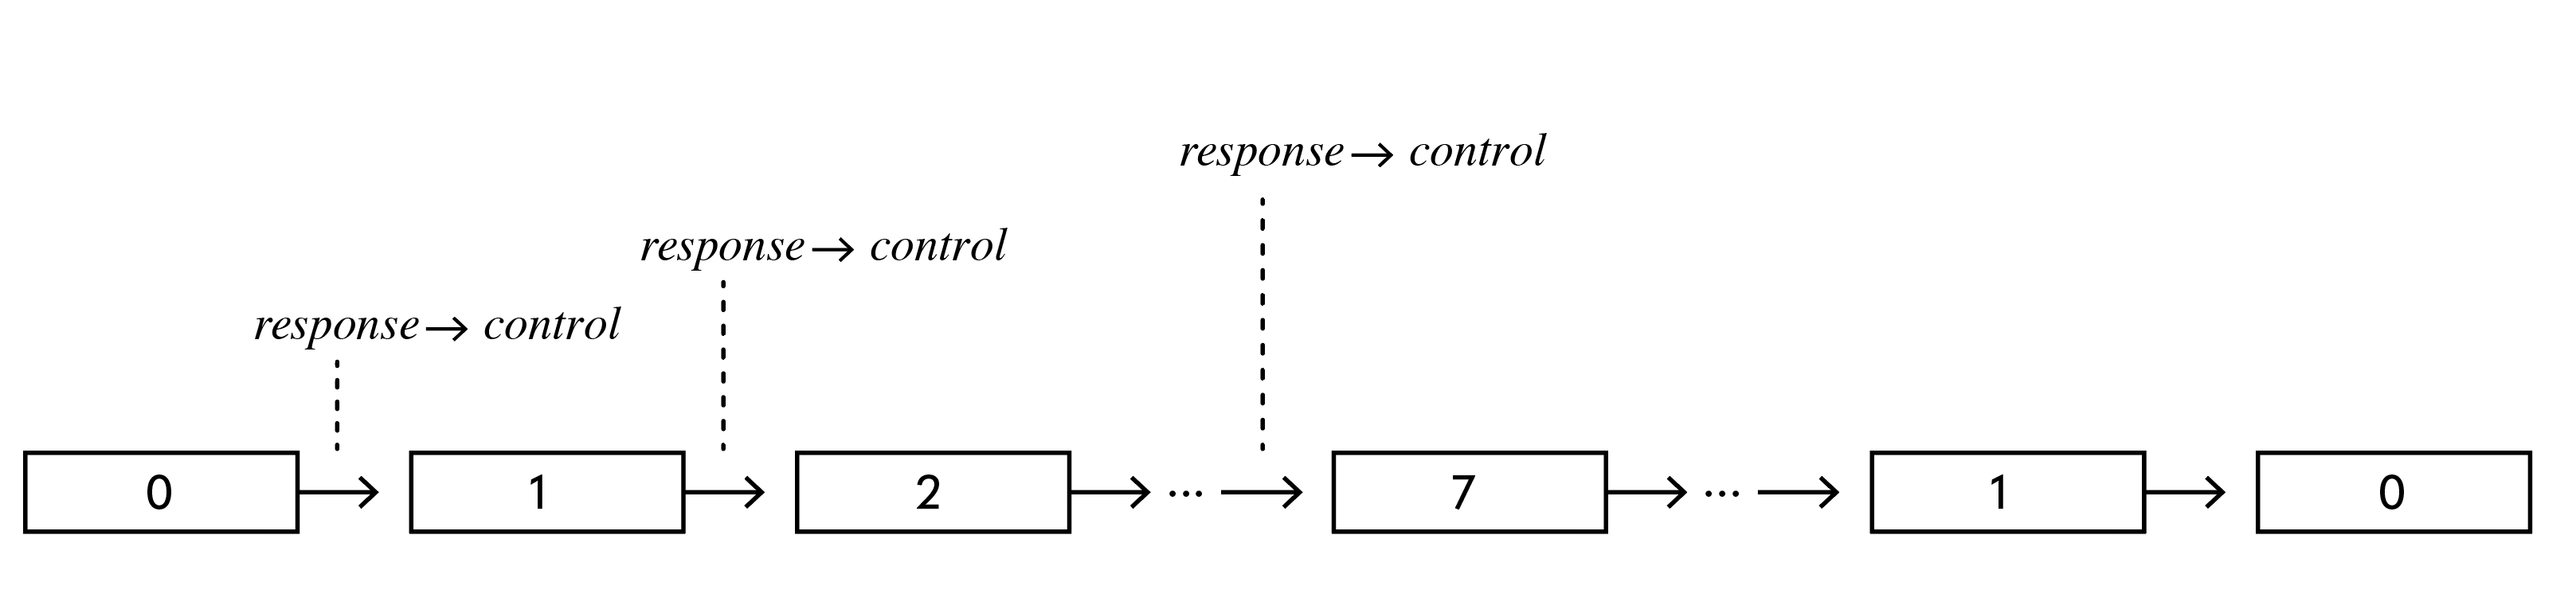
\includegraphics[width=15cm]{img/nerai_fs.png}
  \caption{《Familiar / Strange》のねらい}
  \label{fig:nerai_fs}
\end{figure}

最初、手指が鏡合わせのように表示された状態から始まり、ゆっくりと指一本一本の単位で分割されていく(シーン0からシーン1)。その瞬間に、見慣れていたはずの手指の動きが見慣れないものに感じられ、実際の手指と画面の手指との関係が、Felsの\textit{response}や\textit{contemplation}といった関係性に変化する。2つ目の作品と比べると、ゆっくりとしたテンポで手指の形状が変化する。そのためしばらくすると変化した手指の構造での身体動作を見出し、身体の動かし方が変化することで\textit{control}の関係に至ると考えた。またそれが別の形に変化していくと再び関係性が変化し、その都度、構造に合わせて手指の動かし方が変化していくと考えた。また、バネ状に指の動きが連結されたとき(シーン7)には、はじめて指の動きが相互に干渉するようになり複雑度が増す。そのとき、ある形や運動を生み出すことに「目的の創発」が起き、\textit{control}に加えて\textit{belonging}がおき、一体感が芽生えるのではないかと考えた。

\subsection*{Relation}
この作品におけるねらいは、ボールの操作やマトに当てるといった目的意識が起点となって意識的な試行が引き出され、その目的を達成するための技量を身につけることで一体感が生起することである(図\ref{fig:nerai_rl})。ボールは手指のように直接動かすことができないため、目的意識が生じてもそれを即座に達成することができない。身体の動かし方を画面内の構造にあわせて変化させるだけでなく、ボールの動きを制御するための、より緻密な運動の統合が求められる。このようにして、巧みさを獲得することでボールが思い通りに動かせるようになる(\textit{control})ことで、一体感を感じるのではないかと考えた。またこの作品では、手そのもの、手とボール、ボールとマト、というように、段階的に緻密な運動の制御が求められることで、一体感が高まるのではないかと考えた。
% ボールと手の関係に注意が向いた途端、手指に感じる違和感や注意は向きづらくなる。さらに、マトが現れると、さらにその目的意識は強固になると考えた。これまでの展示の様子から、ボールと手指だけの関係性であっても、まずは飛ばしてみる、転がしてみる、落とさないように気を付けるといった目的意識を設定しやすい。その一方で、手指のみの状態から手指とボールとの関係性に切り替わったときと同様に、マトが出現することがそうした注意を不可視にしてしまうことがこれまでの展示の中で見受けられた。

% そのため、手指の変換、皮膜の出現、ボールの出現、そしてマトの出現は、それぞれタイミングを分けて出力するように調整した。本作はダイナミックな構造の切り替わりこそ少ないが、手指を取り巻く関係性が次々に変化する作品として構成された。そうすることで、それぞれの関係性において異なる注意が生じ、段階的に目的意識が強固になっていくことで、「マトにボールを当てる」という強い目的意識とその達成のための試行錯誤を通して、強い一体感が生じるのではないかと考えた。

\begin{figure}[H]
  \centering
  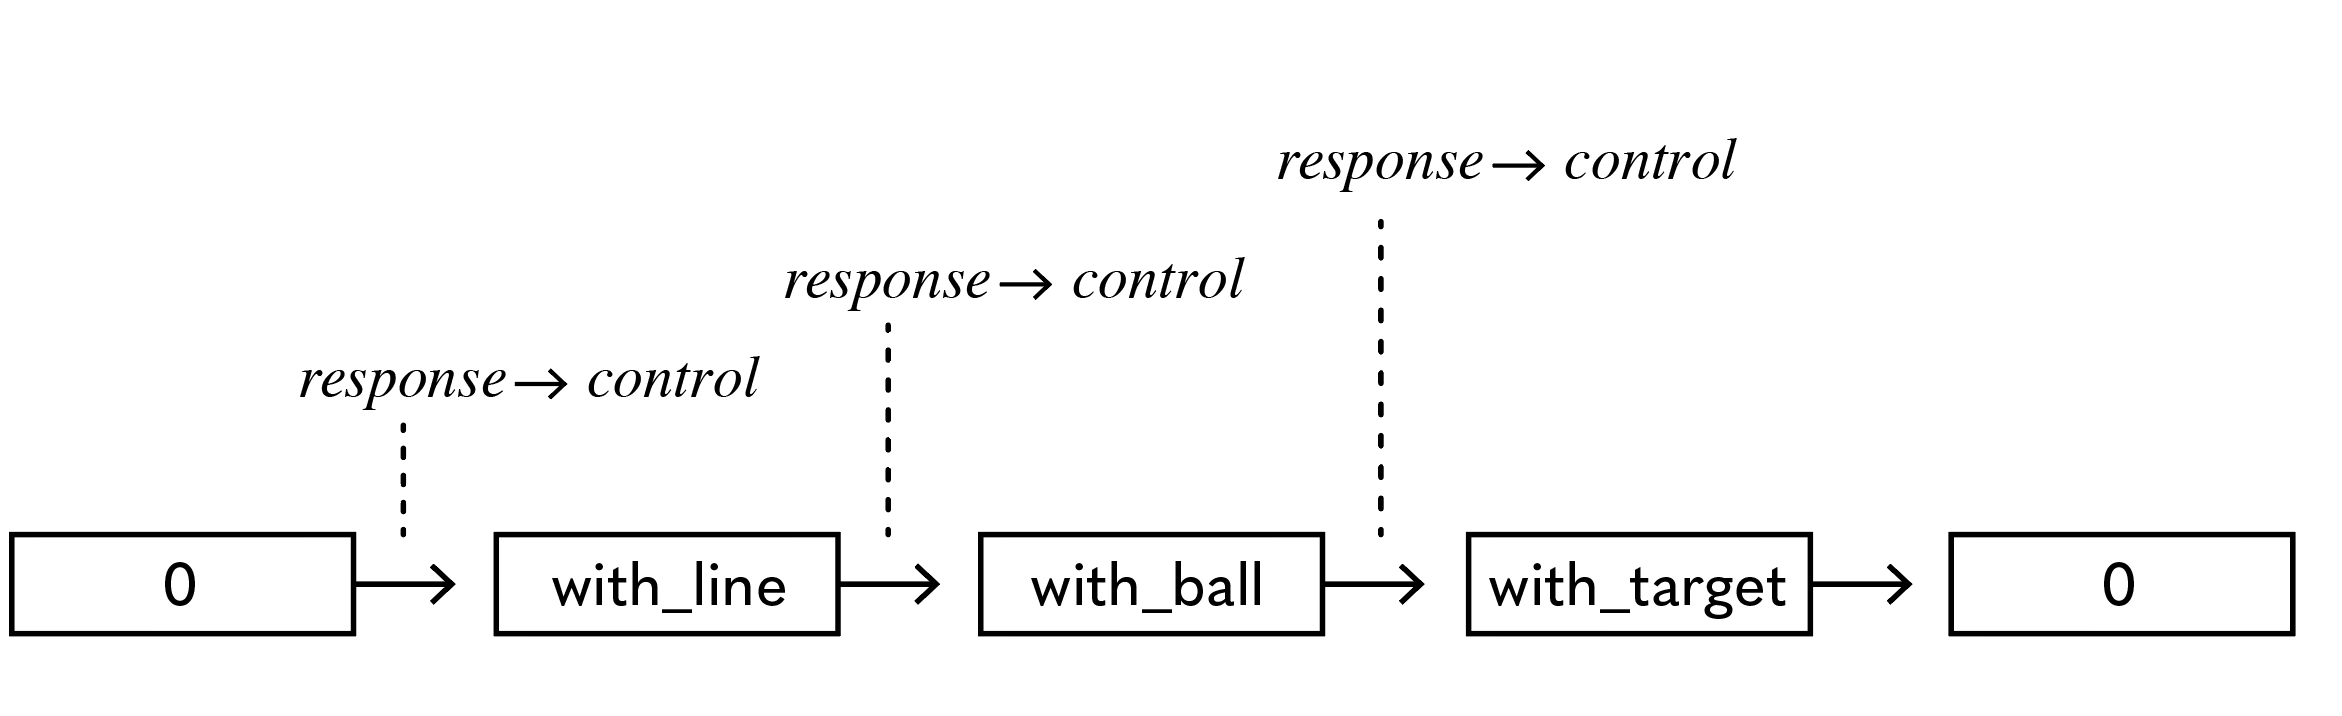
\includegraphics[width=15cm]{img/nerai_rl.png}
  \caption{《Relation》のねらい}
  \label{fig:nerai_rl}
\end{figure}

% \textit{grasp}には二つの性質がある。一つは、時間幅が注意を向けている対象によって、長い場合と短い場合があることである。目的意識が芽生えてからスムーズに操作できるようになる場合、'reach'から'manipulate'が近く、\textit{grasp}は短い、すなわち直感的で使いやすいものとして経験される。その一方、目的意識が芽生えてから試行錯誤を伴い、習熟に長い期間を要する場合、\textit{grasp}は長く、もどかしさを経験し、操れるようになった時に達成感を経験する。\\

% 二つ目に、\textit{grasp}の過程で他のことに対する意識が次々と芽生えることがある。具体的には「やってみるまでわからない」といった経験や、物事に対する解像度が高まる中で、当初とは異なる意識が芽生える状況に相当する。\\

% このコンセプトを展開し、「試行錯誤の余地」を設計することを目指したのが、修士作品《Grasp(er)》である。この作品では、\textit{grasp}を経験する中で、個人による創造的な活動が生まれ、\textit{grasp}という動作を行っているのではなく、そこに'er'の接尾辞がついた'Grasper'であると名付けた。